\graphicspath{{system_design/fig/}}

\chapter{System Design}
\label{chap:system_design}

\begin{figure}[!h]
  \centering
  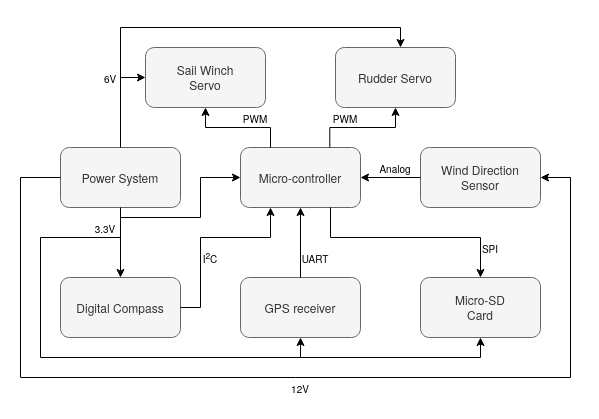
\includegraphics[width=0.918\linewidth]{system_diagram.png}
  \caption[System Diagram]{System Diagram}
  \label{fig:system_diagram}
\end{figure}

\section{Sail Vessel}
The sailing vessel houses the entire system illustrated in Fig. \ref{fig:system_diagram}. Designing and developing a sailboat is a complex task on its own, 
requiring expertise and experience in many fields, some of which include aerodynamics, hydrodynamics and material design. Given the complexity of this task 
and the time constraints of the project, an existing RC sailboat was used. A Dragonflite 95 RC sailboat was modified to incorporate the system illustrated 
in Fig. \ref{fig:system_diagram}. The Dragonflite is 950 mm in length and has an overall weight of two kilograms. It features two sails (mainsail and jib), 
carbon fibre mast and moulded carbon fibre keel with zinc alloy ballast bulb. The sailboat is operated
with a 2.4Ghz 4-channel digital proportional transmitter which communicates with a 2.4Ghz 4-channel receiver. The sail winch servo controls both the mainsail 
and the jib simultaneously. The receiver and two servo motors are powered with a 6v battery source (4 AA batteries). The transmitter and receiver were 
removed as they are not needed in the development of a autonomous sailboat.

\section{Wind direction sensor}
The direction of apparent wind is needed to determine the optimal positioning of the sails. Wind direction sensors that were considered where: an ultrasonic 
anemometer, a mechanical wind vain, and the development of a wind direction sensor using four electret microphones and correlating the signals. The ultrasonic
anemometer that was considered was the WS303U by Sentec Meteorology, it was not used because it is too large for the sailing vessel. The development of a 
wind direction was not done because of the time constraints of the project. The mechanical wind vain was chosen as the most viable option. The sensor used was 
the FST200-202 made by firstrate sensor company. This sensor is designed for outdoor environments such as weather stations and boats, it therefore has 
excellent resistance to extreme weather conditions and erosion. The sensor works in wind speeds greater than 0.8 m/s, has a $22.5^{\circ}$ resolution and 
$\pm 3^{\circ}$ accuracy. It features automatic temperature compensation and operates in a temperature range of $-20^{\circ}C$ to $+85^{\circ}C$. The 
sensor has a working voltage of 12~30VDC, and its output is a 4-20 mA signal. 

\section{Servo motors}
Two servo motors are required: one for controlling the mainsail, and the other for controlling the rudder. The servo motors used were the ones that came with 
the Dragonflite 95, as the vessel was designed to use them; it also kept costs low. The manual specifies that a metal geared servo is used for rudder control
and a sail winch servo is used to control the sail position. Aside from this, no other information is given in the manual about the servo motors.  

\section{Micro-SD card}
The Micro-SD card is used for data-logging purposes, it allows for data from tests to be stored and analysed at anytime. Data that is logged during water tests 
include: current position, current bearing, desired bearing, bearing error, distance to target, wind direction, and tracking speed. A micro-Sd card socket made 
by Pololu was used, and features a SPI communication.  

\section{Power system}
The power system consists of three separate power sources. The rudder servo and sail winch servo are powered by a 6v battery source consisting of four 1.5V
alkaline batteries in series. The Adafruit feather is powered by a 5000mAh 3.7V lithium polymer battery. The Adafruit feather is used to power the micro-SD 
card socket, GPS receiver, and digital compass. The wind direction sensor is powered with two 9V alkaline batteries in series. %Discuss reason you used three
%different power sources instead of one. could say low cost?

